\chapter{Programação por Restrições}
\label{cp:pr}


A programação por restrições (PR) é um paradigma de programação, tal como o paradigma imperativo, o orientado a objetos, o funcional, o lógico e outros. A ideia geral da PR, conforme \cite{thom}, é de resolver problemas simplesmente declarando restrições que devem ser satisfeitas pelas soluções destes.

De acordo com \cite{apt}, a PR já foi aplicada com sucesso em diversas áreas, como biologia molecular, engenharia elétrica, pesquisa operacional e análise numérica. Entre as principais aplicações, pode-se citar sistemas de suporte à decisão para problemas de escalonamento e alocação de recursos \cite{thom}.

Problemas que hoje são identificados como sendo de satisfação de restrições, como por exemplo programar os horários de trabalho em uma empresa, sempre estiveram naturalmente presentes de alguma forma com a humanidade. Entretanto, métodos específicos para solucionar este tipo de problema começaram a surgir no meio acadêmico apenas nas décadas de 1950 e 1960, apesar de que técnicas como o \textit{backtracking} (um método de busca exaustiva refinado) já eram utilizadas de forma recreativa desde o século XIX \cite{cphandbook}.

A Seção \ref{sc-conceitos-basicos-pr} apresenta alguns conceitos básicos deste paradigma, de forma a esclarecer como este funciona e o que o difere do paradigma imperativo. A Seção \ref{sc-modelagem} esclarece as propriedades da modelagem de problemas por meio de uma linguagem de PR. A Seção \ref{sc:minizinc} apresenta a linguagem MiniZinc e demonstra alguns recursos da linguagem com o auxílio de um exemplo.



\section{Conceitos Básicos}
\label{sc-conceitos-basicos-pr}

Algumas definições de termos comumente utilizados na área são apresentadas em \cite{leler}. Conforme este, uma restrição expressa uma relação desejada entre um ou mais objetos. Uma linguagem de PR é uma linguagem que possibilita descrever os objetos e as restrições. Um programa feito em uma linguagem de PR define um conjunto de objetos e um conjunto de restrições sobre estes objetos. Um sistema de satisfação de restrições encontra soluções para programas feitos em uma linguagem de PR, ou seja, atribui valores aos objetos de forma que todas as restrições sejam satisfeitas.

Conforme \cite{stuckey}, as restrições presentes no mundo real podem ser modeladas por meio de restrições em linguagem matemática. Desta forma, os objetos que tais restrições relacionam são também de cunho matemático, tais como variáveis e números.

Um exemplo simples apresentado em \cite{leler} é a conversão de temperaturas. Por exemplo, a restrição:
\[
  C = (F - 32) \times \frac{5}{9}
\]
define o relacionamento entre temperaturas em Fahrenheit e Celsius, representadas respectivamente pelas variáveis $C$ e $F$.

Em \cite{leler}, também é reforçado o fato de que o sinal de igualdade em linguagens de PR possui o mesmo sentido da igualdade matemática. Isto difere-se de grande parte das linguagens imperativas (por exemplo C, Java e Python), nas quais o sinal de igualdade representa a operação de atribuir um valor a uma variável. Desta forma, em uma linguagem de PR, a restrição acima poderia ser reescrita, por exemplo, da seguinte forma:
\[
  9 \times C = 5 \times (F - 32)
\]

Como tal restrição descreve o relacionamento entre as variáveis $C$ e $F$, a partir do momento em que uma das variáveis receber um valor, o valor da outra variável já pode ser calculado. Além disto, caso fosse necessário realizar conversões para a escala Kelvin, bastaria adicionar a seguinte restrição:
\[
  K = C - 273
\]

em que $K$ é a variável que representa a temperatura em Kelvin. Assim como na restrição anterior, caso o valor de uma das variáveis for conhecido, o valor da outra pode ser calculado. Além disto, as restrições pertencentes ao conjunto de restrições de um dado programa são dependentes entre si. Desta forma, apenas com estas duas restrições é possível converter temperaturas entre Kelvin e Fahrenheit, sem explicitar a fórmula de conversão entre tais unidades \cite{leler}.

Entretanto, as restrições não se limitam à equações lineares. Os tipos de restrição e de domínios de variáveis variam dependendo da linguagem. Os tipos comuns de domínio de variáveis são, por exemplo, inteiros, reais, booleanos, conjuntos, vetores, e outros. Também se faz possível declarar inequações, por exemplo, por meio dos operadores $\ge$ e $\not=$.

As operações possíveis entre as variáveis também variam, mas normalmente se faz possível utilizar as operações aritméticas básicas, como $+, -, /, \times$, para inteiros e reais, operadores lógicos, como $\wedge, \vee, \rightarrow, \leftrightarrow$, para booleanos, operações como $\cup$ e $\cap$ para conjuntos, entre outros.

Outro tipo de domínio de grande importância para a PR são os domínios finitos. Os valores possíveis que uma variável de domínio finito pode receber são restritos a um conjunto finito de valores. Um exemplo clássico de domínio finito é o domínio booleano, no qual as variáveis só podem receber os valores \textit{true} ou \textit{false}. Outro exemplo são os intervalos de valores inteiros, como $[1,10]$, por exemplo.

Os domínios finitos são amplamente utilizados na PR por permitirem ao programador modelar de forma natural problemas que envolvem escolhas, representando cada uma das possíveis escolhas por meio dos valores presentes no domínio \cite{stuckey}.



\section{Modelagem}
\label{sc-modelagem}

\cite{kowalski} afirma que os algoritmos possuem dois componentes distintos, a lógica e o controle. A lógica está relacionada com o que o algoritmo faz, o conhecimento que se possui sobre o problema. O controle, por sua vez, representa como tal lógica será utilizada para resolver o problema.

No paradigma imperativo, geralmente não há uma distinção clara entre tais componentes, visto que os problemas são resolvidos seguindo uma sequência de instruções, que fazem tanto parte do controle quanto da lógica propriamente dita \cite{thom}.

Uma das vantagens do paradigma declarativo, do qual a PR faz parte, é a possibilidade de focar de forma praticamente exclusiva no componente lógico, sem se preocupar com o controle \cite{thom}.

Desta forma, para se resolver um problema utilizando o paradigma de PR, basicamente se faz necessário apenas modelá-lo matematicamente em termos de váriaveis e restrições. Apesar de não ser uma tarefa trivial, em muitos casos fazer tal modelagem é muito mais simples do que desenvolver um algoritmo utilizando o paradigma imperativo, visto que neste último se faz necessário explicitar cada passo necessário para a resolução do problema, enquanto que com a PR basta descrever o problema.

Conforme \cite{stuckey}, um problema de satisfação de restrições pode ser formalmente modelado por meio de uma restrição $C$ sobre váriaveis $x_1, ..., x_n$, e um domínio $D$ que mapeia cada variável $x_i$ ao conjunto finito de valores que esta pode assumir. Tal restrição $C$ é a conjunção de todas as restrições definidas.

Após o desenvolvimento de um programa em uma linguagem de PR, para se obter as soluções do problema, se faz necessário utilizar um sistema de satisfação de restrições (\textit{solver}). De acordo com \cite{cphandbook}, tais sistemas utilizam diversos métodos para atribuir valores às variáveis de forma a satisfazer todas as restrições. Entre estes métodos, pode-se citar o \textit{backtracking}, \textit{branch and bound} e a propagação de restrições, que não serão apresentados em detalhes neste trabalho.

Em alguns casos, além de ser necessário satisfazer todas as restrições de um problema, também se faz preciso otimizar a solução deste. Nestes casos, além de se definir o conjunto de variáveis e de restrições, define-se também uma função objetivo a ser otimizada (maximizada ou minimizada). Tal função objetivo mapeia cada solução do problema em um valor real, possibilitando assim definir qual é a solução mais otimizada \cite{apt}.

\subsection{Exemplo de Modelagem}
\label{ss:exemplo-de-modelagem}

Um dos exemplos clássicos utilizados para ilustrar a PR é o famoso problema das $n$-rainhas. O objetivo deste problema é posicionar $n$ rainhas em um tabuleiro $n \times n$ de xadrez, com $n > 3$, de tal forma que as rainhas não se ataquem mutuamente \cite{apt}.

Uma das modelagens mais comuns para este problema, apresentado em \cite{apt}, é representar a posição de cada uma das $n$ rainhas por meio de variáveis $x_1, x_2, ..., x_n$, sendo o domínio de tais variáveis $[1,n]$. O valor de cada variável $x_i$ indica qual é a linha em que está a rainha que se encontra na coluna $i$.

Para o tabuleiro apresentado na Figura \ref{fg:8-queens}, que demonstra uma possível solução para o problema com oito rainhas, o valor das variáveis $x_i$ é respectivamente $6, 4, 7, 1, 8, 2, 5, 3$. Tais valores foram calculados assumindo a primeira coluna como sendo a mais a esquerda e a primeira linha como sendo a mais abaixo.

\begin{figure}[!ht]
  \centering
  \caption{Uma possível solução para oito rainhas}
  \label{fg:8-queens}
  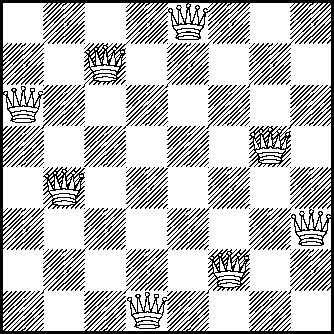
\includegraphics[width=0.35\textwidth]{figuras/8_queens.png}
  \\ Fonte: \cite{apt}
\end{figure}

Para garantir que as rainhas sejam posicionadas de forma a não se atacarem, se faz necessário declarar um conjunto de restrições sobre as variáveis $x_i$. As desigualdades a seguir são suficientes para garantir que os valores de tais variáveis formem uma configuração válida conforme o objetivo do problema, para $i \in [1,n-1]$ e $j \in [i+1,n]$:

\begin{itemize}
  \item $x_i \not= x_j$
  \item $|x_i - x_j| \not= |i - j|$
\end{itemize}

A primeira desigualdade impede que duas ou mais rainhas sejam posicionadas na mesma linha. Tal desigualdade gera um total de $\frac{n(n-1)}{2}$ restrições ao se aplicar todos os possíveis valores de $i$ e $j$. Todas estas restrições juntas garantem que todas as variáveis assumirão valores distintos entre si.

A segunda desigualdade impede que duas ou mais rainhas sejam posicionadas na mesma diagonal. Assim como para a primeira desigualdade, esta também gera um total de $\frac{n(n-1)}{2}$ restrições ao se aplicar todos os possíveis valores de $i$ e $j$, gerando assim um conjunto com $n(n-1)$ restrições ao todo.

Não se faz necessário restrições para verificar se duas ou mais rainhas estão posicionadas na mesma coluna, visto que a forma como o tabuleiro foi modelado já impede naturalmente que tal situação aconteça.